\documentclass[10pt,twocolumn,letterpaper]{article}

\usepackage{iccv}
\usepackage{times}
\usepackage{epsfig}
\usepackage{graphicx}
\usepackage{amsmath}
\usepackage{amssymb}
\usepackage{listings}
\usepackage{verbatim}
\usepackage{algorithm2e}
\usepackage{cite}

\long\def\sw#1{\textcolor{red}{**[SW] #1**}}
\long\def\ge#1{\textcolor{green}{**[GE] #1**}}
\long\def\dv#1{\textcolor{blue}{**[DV] #1**}}

\newcommand{\obs}{\mathbf{O}}
\newcommand{\state}{\mathbf{X}}
\renewcommand{\vec}[1]{\ensuremath{\overrightarrow{#1}}}


% Include other packages here, before hyperref.

% If you comment hyperref and then uncomment it, you should delete
% egpaper.aux before re-running latex.  (Or just hit 'q' on the first latex
% run, let it finish, and you should be clear).
\usepackage[pagebackref=true,breaklinks=true,letterpaper=true,colorlinks,bookmarks=false]{hyperref}

 %\iccvfinalcopy % *** Uncomment this line for the final submission

\def\iccvPaperID{****} % *** Enter the ICCV Paper ID here
\def\httilde{\mbox{\tt\raisebox{-.5ex}{\symbol{126}}}}

% Pages are numbered in submission mode, and unnumbered in camera-ready
\ificcvfinal\pagestyle{empty}\fi
\begin{document}

%%%%%%%%% TITLE
\title{Hard real time multi person detection}

\author{Deepak Geetha Viswanathan\\
University of Amsterdam\\
Science Park 904, Amsterdam\\
{\tt\small D.GeethaViswanathan@uva.nl}
% For a paper whose authors are all at the same institution,
% omit the following lines up until the closing ``}''.
% Additional authors and addresses can be added with ``\and'',
% just like the second author.
% To save space, use either the email address or home page, not both
\and
Gwenn Engelbienne\\
University of Amsterdam\\
Amsterdam\\
{\tt\small g.englebienne@uva.nl}
\and
Shimon Whiteson\\
University of Amsterdam\\
Amsterdam\\
{\tt\small s.a.whiteson@uva.nl}
\and
Ben Krose\\
University of Amsterdam\\
Amsterdam\\
{\tt\small b.j.a.krose@uva.nl}
}

\maketitle
%\thispagestyle{empty}


%%%%%%%%% ABSTRACT
\begin{abstract}
Trained object detectors are an important component of tracking by detection systems. For robust localization and tracking, computationally expensive detectors are needed, but are these are not usable in practice in an online setting.  In this work, we describe a novel multi person detection framework based on quantifying the uncertainty of camera observations at different world locations, and using it to prune the search space of a parts based detector. Online settings force us to adhere to hard computational constraints. By making smart choices about which windows to select in every image, we utilize the maximum potential of the parts based detector within the available computational resources. 
 This framework enables us to compute an accurate belief about the location of the people in the environment using a pruned set of input locations, thus reducing the computational load on the detection system and making accurate online tracking in challenging environments feasible in practice.
\end{abstract}

%%%%%%%%% BODY TEXT
\section{Introduction}
Multi-person detection is a key problem in computer vision.  In addition to its direct applications, in e.g., \sw{add examples with cites}, detection is also important as a subroutine in person tracking \sw{cite} frameworks.  

A key challenge in multi-person detection is to develop methods that work well in on-line settings in which hard computational constraints must be obeyed. For example, a mobile robot may require real-time  estimates of the location of people in its environment in order to perform socially aware navigation.  In such settings, high-quality detection often necessitates multiple cameras.  The volume of data generated by these cameras is then difficult to process within the given computational constraints.  

Existing state-of-the-art systems typically use either \emph{detection by background subtraction} \sw{cite} or \emph{detection by classification}~\cite{Pami-11}.

Background subtraction methods~\cite{bk1}~\cite{bk2-bayesian} are computationally inexpensive and can be used online. However, they have poor accuracy in realistic environemnts because they can only detect people when they are in motion. 
Moreover, while background subtraction methods can cope with diversity in the poses and appearances of the people in the foreground, they provide no principled way to interpret this foreground. Such methods have difficulty determining which parts of the foreground are actually touching the ground and therefore mapping the observations in the image domain to the world domain.

By contrast, detection by classification methods are typically much more accurate because they explicitly model the foreground, i.e., the overall shape of the person~\cite{dalaltriggs} as well as individual body parts~\cite{DPM}~\cite{partsDeva}.  Sophisticated parts-based models in particular can provide robust detection in real world environments.  However, these models introduce high computational costs that preclude the use of such methods in online settings.

In this paper, we present a new approach for multi-person detection that gets the best of both worlds.  In particular, it approaches the accuracy of parts-based detectors but with much lower computational costs.  Furthermore, because it can obey hard computational constraints while making efficient use of whatever computational resources are available, it is ideally suited to on-line settings.

The main idea is to quantify the system's uncertainty about people's locations and use this to make smart choices about where to apply the expensive parts-based detector.  In the off-line phase, we learn observation models for each detector that estimate the probability of detection given people's true locations.  In the on-line phase, we apply the background subtraction detector to the whole image collected by the camera and, using its observation model, compute a posterior distribution over people's locations.  Then, using this posterior and the observation model for the parts-based detector, we select a subset of the windows in all the images that are estimated to maximize \emph{information gain}.  We then apply the parts-based detector only to this subset and use the resulting detections to compute a second posterior, from which final predictions about people's locations can be made.  By making smart choices about where to apply the expensive detector, this method can achieve high accuracy at much lower computational cost.  In addition, since it works with window subsets of any size, it can easily be tuned to meet hard computational constraints.  

We evaluated our method on a real-world dataset gathered from a multi-camera system \sw{Is it still multi-camera?} consisting of \sw{add details.}  Our results show that our method performs nearly as well as, but is much faster than, a standard parts-based detector.  In addition, it substantially outperforms baselines that use only background subtraction detectors or that naively combine both detectors.

\section {Related Work} \dv{To Edit}

%Motivate tracking by detection
Trained object detector is widely used for practical tracking scenarios~\cite{Pami-11}~\cite{POM-main}~\cite{MIL-obj1}. Background subtraction methods~\cite{bk1}~\cite{bk2-bayesian} are used far less in state of the art systems. Object detectors are more tolerant to illumination variations~\cite{ObjDet-1} and also can detect static people. Robust tracking systems can be built using  tracking by detection framework.

%Motivate Parts based models and their importance in tracking
Different techniques are available for detection with varying computational requirements. Until recently, overall shaped based models where used more predominantly as the object detectors, but in recent literature, the use of parts based models of the person is being explored~\cite{doubleperson}~\cite{Parts_tracking1}.
In ~\cite{Parts_tracking1}, they use the DPM model for tracking in difficult multi target scenarios. They exploit the potential of individual part detectors to reason about occlusions dynamically. In ~\cite{doubleperson} occlusions are handled using a specially trained detector to detect partially occluded pair of people. 
Altough these methods are applicable online, the computational cost of applying the parts detector is a concern. One of the requirements in using parts based models in tracking is the availability of high resolution data of the environment. Altough sensors which can provide such data is widely available, the applicability of parts based detectors in an online setting is a problem which is not addressed in any of the works. This is a shortcoming we have rectified in our work. 

%Motivate observation function
Another aspect of using the tracking by detection framework is to tranform the sliding window outputs to a useful likelihood function which can be used by a time dependent tracking framework. This is an important aspect of using trained detectors.  Conventional approaches of using a non maximal suppression and modelling the likelihood using suppressed detections throws away a large amount of information provided by the detector in an ad-hoc way. This reduces the efficiency of the bayesian tracker which then uses the non-maximally suppressed output. In ~\cite{POM-main} all the detections from different locations are used to build a probablistic likelihood map. The idea of using a more descriptive likelihood is used in several recent works. In ~\cite{Pami-11} the authors use the confidence values of the detector at different image locations for creating a likelihood function which they later use for particle filter based tracking. In our work, we emphasize the importance of a learnt observation model for transforming the detector results. Performance of standard detectors on a specific environment is highly variable depending on illumination conditions, density of crowd, height of camera placement, and many other factors which cannot be explicitly quantified. The most general way of being able to apply standard detectors on various environments is to quantify the performance of the detector using domain specific data by learning an observation model. Section 5 explains the generic observation model which can be learnt from labelled data.

%Motivate action selection
The problem of dynamic resource allocation has been widely researched in the area of sensor networks. We can classify the exisisting techinques into non-myopic and myopic planning techniques.  Decision theoretic framework of POMDP~\cite{Kaelbling98}, provides a theoretically sound backbone for incorporating non myopic control in bayesian systems. Dynamic planners using POMDP have been successfuly used in sensor selection scenarios~\cite{Spaan09}, where optimal selection of cameras using temporal planning (given a  fixed computational budget) can provide a performance benefit over greedy sensor selection. In more complex scenarios, where it is not tractable to solve the large state-action spaces using POMDP (temporal planning methods), more pragmatic yet principled methods such as subodularity based greedy action selection have also proved to provide gauranteed performance benefits. In ~\cite{krause2012near} they propose the idea of using information gain as an objective function for the subset selection problem. They also prove that information gain as objective function is submodular. Nevertheless, the idea of resource allocation in high level computer vision algorithms is still an under explored area.Specifically, what we are interested in is a budgeted use of the outputs of the sensors (or detectors), in a principled way so as to not losing on the tracking performance. We exploit the submodularity property of information gain for smart use of the computationally expensive parts based detector.


\section{Problem Setting}


We consider an indoor environment in which $ n$ people move throughout a ground plane that is discretised into cells.  At most one person can occupy each cell at a time. We want to track the people using a wide field of view, calibrated, omni-directional camera. The camera is mounted on the ceiling facing the ground plane, with the camera axis perpendicular to the ground plane.

The \emph{state} of the world is described by a vector $\mathbf{X}$ of length $n$, where each $X_i$ is a binary variable indicating whether cell $i$ is occupied. $|\mathbf{X}| $ is the total number of cells. 

For each cell, the projection of the shape of a person in the image can be approximated by a rectangular window. This rectangular sub-image or \emph{window} at cell $ i $ is represented by $ I_{i} $. The windows are extracted and evaluated by a \emph{detector}. The quality of the overal perception depends on the subset of the cells to which the detector is applied and the location of the people in the environment.

Our goal maintain a posterior distribution or \emph{belief} over $\mathbf{X}$.  While the background subtraction detector can be applied to all windows, computational constraints allow us to apply the parts-based detector to only $K < |\mathbf{X}|$ windows.  Therefore, in the next section, we propose a framework for accurately and efficiently maintaining a belief over $\mathbf{X}$ by making smart choices about the $K$ windows to which we apply the parts-based detector.  Table \ref{tab:Formal symbols} summarizes the notation used to describe the problem setting.

\begin{table}[ht] 
  \begin{tabular}{lll}
   \hline
   Symbol & Explanation \\
   \hline
   $\textbf{G} $ & Number of cells\\
   %$G_{c} $ & Set of all cells visible from camera $c$.\\
   $ \textbf{I} $ & Raw input image from camera.\\
   $ I_{i} $ & Raw image at location (Window) $ i$\\
   %$ W_{i}^{c} $ & Window at location $ i$\\
   $ \textbf{O} $ & Observation map - Classifier output for all  $ i $\\
   $O_{i} $& Detector output for all $ i $\\
   $\textbf{X}$& True state (occupied/not occupied) for all $i$\\
   \hline
  \end{tabular}
  \caption{%
    Problem setting notation. \sw{This table is out of date and contains notation that was not introduced in the text.}
  }
  \label{tab:Formal symbols}
\end{table}

\section{Proposed Framework}

\begin{figure*}
\begin{center}
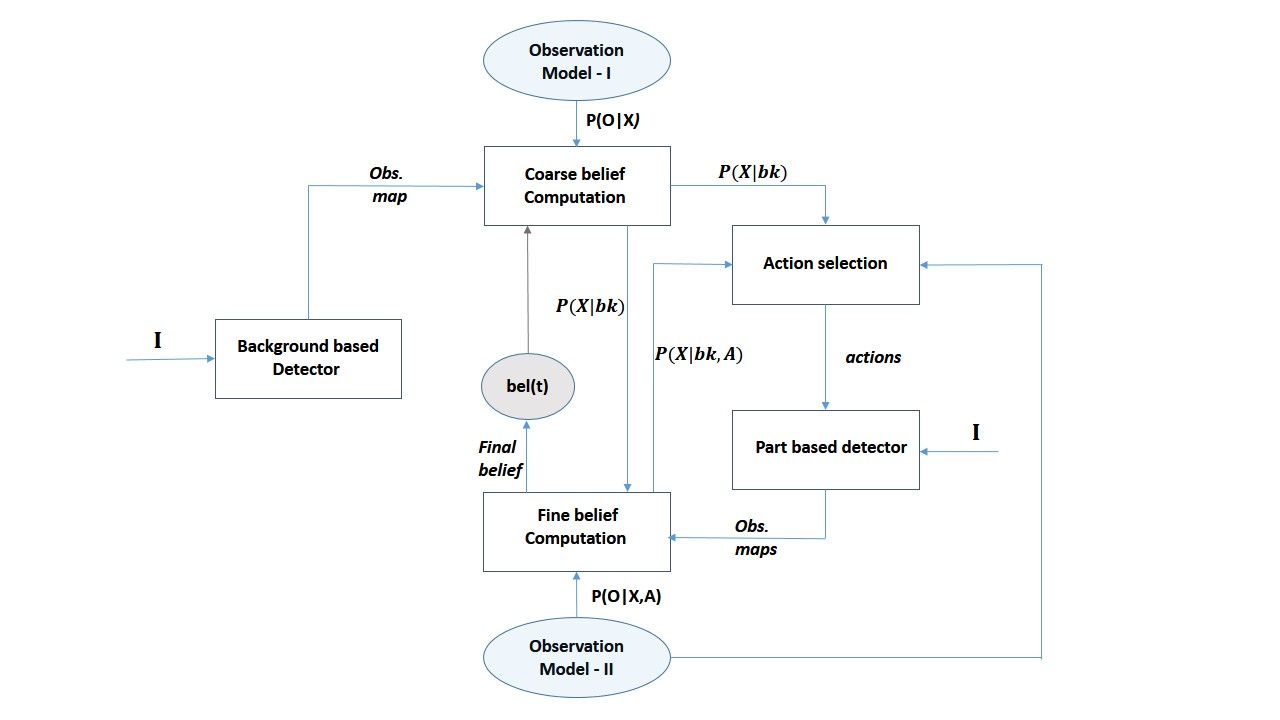
\includegraphics[width=12cm]{img/newBlockdia.jpg}
\end{center}
   \caption{A schematic diagram of the proposed active data fusion system}
\label{fig:Block dia}
\end{figure*}

Our framework consists of two phases.   In the \emph{off-line phase}, the detectors and their corresponding observation functions are trained.  In the \emph{on-line phase}, a belief about $\mathbf{X}$ is iteratively updated using observations gathered from applying the background subtraction detector to all windows and applying the parts-based detector a carefully selected subset of the windows.

\subsection{Offline Phase}
 
 \subsubsection{Detectors}
We study the use of two contrasting detectors. The first one is a background based detector and the second one is a parts based detector.

A template based probabilistic model is used as the background based detector\cite{englebienneFast}. It works in real time and has a grid based approach which makes it suitable for our setting.

We have used the the non articulated flexible mixture of parts model\cite{partsDeva} for the parts based detector. Specifically, a 26 part model of the human body which uses small, non-oriented parts is used.
More details of the model parameters used is described in the experiments section.

\subsubsection{Observation model}
In order to compute a meaningful belief about the state, we need to learn an observation model which will quantify the uncertainity in the detector output for different state configurations. An observation model correlates the output of the detector $O_{i}$ to different world states $\textbf{X}$.
We learn this observation model from data for both the background based detector and the parts based detector.
\subsection{Online sequential process}
The online process consists of two main steps for estimating the belief. First is the \textit{coarse belief computation} and the second is \textit{fine belief computation}. The online process is represented in figure \ref{fig:Block dia}.
At time $t $, an image is acquired from the camera. The background based detector is applied on all the locations in the image. The detector output from the background based detector is used to create an \textit{observation map}, $\textbf{O}$. An observation map is the detector output for all cells in the ground plane.  

The next step is the coarse belief computation. Using the observation map and the learnt observation model for the background based detector, we compute a coarse belief about the location of the people in the world (state) using MCMC sampling.
Once we have estimated a coarse belief, we perform the fine belief computation using this belief as a prior.
For the fine belief computation, based on our computational budget, we have multiple \emph{intra time steps} over which we re-estimate our belief. 
At the first intra time step, using this estimated state and information gain as objective function, we compute the most informative window location.
We apply the parts based detector in this window and fold in the detector output of the parts based detector for a more accurate belief.
Iteratively at each of the next $K-1$ intra time steps, we pick the most informative window and improve the belief about the location.

The different modules invovled in the system is explained in detail in the following sections.

\section{Observation model}
From labelled multi person data and the detector output for all the locations we learn the probability distribution $ P(\textbf{O}|\textbf{X})  $ of
obtaining an observation from the detector $ O^{c}_{i} $ (that a grid cell is occupied or not occupied), given the true location of all the people in the environment(the true state of the world $\textbf{X}$).

\subsection{Factorization}

The observation model will have very high dimensionality if represented in the naive form. In order to learn a meaningful representation from available data, it would be beneficial to reduce the dimensionality of this observation model.
We can consider that the observations from each grid cell are independent of one another conditioned on the true state.
\begin{align}
P(\textbf{O}|\textbf{X})&=\prod_{i} {P(O_{i}|\textbf{X})}
\end{align}
Next we reduce the dimensionality of state space if we consider only a \textit{neighbourhood} around $ X_{i} $, instead of the whole occupancy $\textbf{X} $. A neighbourhood for cell $i$ is defined as the set of cells which overlap with the cell $i$, when their corresponding windows are considered in the image. The detector output of a window at location $ i $ is only affected by its own occupancy and a neighbourhood of cells which overlaps with the cell at $ i$. This approximation can be represented as follows: 
\begin{align}
  P(\obs|\state) &= \prod_{i} \, P(O_{i}|X_{i},X_{n(i)})
\end{align}
We now need to learn  $ P(O_{i}|X_{i},X_{n(i)}) $. Depending on the values that $ X_{n(i)} $ can take, we have three distinct scenarios of occupancy. In the next subsection we will explain how to model the features of the state that the observation model conditions on, for these three scenarios of occupancy.

\subsection{Feature representation}

As mentioned above, based on the neighbourhood occupancy, we can have three distinct cases : vacant neighbourhood, single person in the nieghbourhood and multiple people in the neighbourhood. Let us consider each of the three cases seperately.
Using a feature transformation function, we convert the the occupancy scenarios to a binary feature. This is explained for each of the scenarios.

\paragraph{Vacant neighbourhood} When the neighbourhood is empty, and when the cell is also not occupied, we have a probablity for false positives.
\begin{align}
 P(O_{i} |X_{i}=0 ,f(X_{n(i)}) =0)  &=\mu^{0}_{0}
\end{align}

In case when a cell is occupied, the probability of detection computed as:
\begin{align}
 P(O_{i} |X_{i}=1 ,f(X_{n(i)}) =0)  &=\mu^{0}_{1}
\end{align}
The functions $ \mu^{0}_{0} $  and $ \mu^{0}_{1} $ is learnt from training data.


If there are multiple people in the neighbourhood, we compute the maximally overlapped neighbour and approximate that the effect of the nieghbourhood on the detector output can be modelled sufficiently accurately using this maximally ovelapped neighbour and ignoring other occupancies of the neighbours. The maximally occupied neighbour $ \textbf{J}_{i} $ is computed as :

\begin{align}
 \textbf{J}_{i}^{c} = \operatorname*{arg\,max}_{j\in n_{c(i)},X_{j}=1} \Vert I_{i}^{c}\cap I_{j}^{c} \Vert  
\end{align}

This approximation is essential to have a tractable dimensionality for the observation model. 
This reduces the possible occupancies of neighbours to two. Either a maximally occupied neighbour or an empty neighbour. 

The four configurations are now straightforward based on the occupancy of the cell $i$ and a maximally occupied neighbour.

In order to generalize these occupancy configurations over the whole state space, we use state features which can appropriately  
model the important aspects of the state space which affects the detector accuracy. This enables us to learn an observation model over these state features from a tractable amount of labelled data instead of each combination of a cell and its neighbour.

%Let us define two features which can quantify the performance of the detectors. The first feature used is the distance of a cell to the camera.
%This is the distance from the centre of the camera projected on the ground plane to the cell $i$ which is to be evaluated.
%\begin{align}
%\alpha(i) = dist(i,camera)
%\end{align}
The first feature used is the overlap between the cells. Cells which are in the nieghbourhood of each other overlap in the image and causes interaction in the detector outputs for those cells. So for such overlapping cells, occlusion is a problem which needs to be modelled. The amount of overlap between the cells is a used as given below. 
\begin{align}
\beta(i,j) = \dfrac{\Vert I_{i}^{c} \cap I_{j}^{c} \Vert}{\Vert I_{i}^{c} \cup I_{j}^{c} \Vert}
\end{align}

Another feature which is essential to incorporate the effect of occlusion is the relative distance of the cells to the camera. 
The impact of occlusion is different when a neighbour is in front of a cell rather than behind it. 
\begin{align}
\gamma(i,j) = \dfrac{dist(i,camera)}{dist(j,camera)}
\end{align}
Now based on these two features, we need to learn the distribution over the possible observations for the four different occupancy configurations.  


Let us consider that one of the neighbours of $ i$ is occupied. This occupancy affects the classifier response at $ i$. The $\beta$ and $\gamma$ parameters described can model this appropriately.
 \begin{align}
 P(O^{c}_{i} |X_{i}=\lambda , j \in{n_{c(i)}},X_{j} =1)  &=\mu^{1}_{\lambda}(\beta(i,j),\gamma(i,j))
\end{align}


For the case of maximally occupied neighbour $ \textbf{J}_{i} $, 
\begin{align}
 P(O^{c}_{i} |X_{i}=\lambda ,\exists j  \in{n_{c(i)}},X_{j} =1)  &=\mu^{2}_{\lambda}(\beta(i,j),\gamma(i,j))
\end{align}

\section{Belief computation}
We are interested in the true occupancy of the state, and this can be computed from a probabilistic belief about the state. Since the state space is large, we resort to sampling based techniques for computing the belief about the state. An MCMC based sampler is used for this purpose.
\dv{Where to add the mcmc sampling details? How do I seperate the action selection and beleif computation sections?}


\subsection{Different beliefs}

At every time step, after we apply the background based detector, we can compute a belief over the state of the world, $P(\textbf{X}|bk)$. Let us denote this by $ P^{0}(\textbf{X})$. 

During the intra time step (while incrementally building the final set of actions), we can compute the posterior distribution over the states based on the currently selected set of incomplete actions, $ P(\textbf{X}|bk,\underline{\mathcal{A}^{k}} )$. Let us denote this by $ P^{k}(\textbf{X})$ ($1 \leq k \leq K $)

After selecting the $K $ actions and observing the detector output corresponding to the actions, we can recompute the posterior distribution, $P(\textbf{X}|bk, \underline{\mathcal{A}^{K}})$. This will be denoted by $P^{K}(\textbf{X})$.

\section{ Action Selection}

\begin{table}[ht]
  \begin{tabular}{lll}
   \hline
   Symbol & Explanation \\
   \hline
$\textbf{X} $ & State of the world\\
 $\mathcal{X} $ & Set of samples of $\textbf{X}$ \\
 $\textbf{W} $ & Set of all possible actions\\
 $K$ & Maximum number of actions in one time step\\
 $\mathcal{A} $ & Set of selected actions\\
 $\mathcal{A}^{k} $ & Set of selected actions at intra time step $k$\\
 $\underline{\mathcal{A}} $ & Detector results corresponding to $\mathcal{A}$\\
 $a $ & An action\\
 $ \underline{a} $ & Detector results corresponding to $ a$\\
   \hline
  \end{tabular}
  \caption{
    Symbols - action selection
  }
  \label{tab:Symbols in action selection}
\end{table}



We need to incrementally build a set of actions of size $ K $, where $ K $ represents our computational budget for applying the parts based detector at every time step. 

We solve this problem using greedy maximization over all possible actions with respect to a metric such as information gain. We use information gain to quantify the "value" of all possible actions and then incrementally build the set of actions greedily.
We need to compute $I^{k}(\textbf{X};a)$ and pick the $a$ which maximizes the information gain. More formally,

\begin{align}
a^{k} = \operatorname*{arg\,max}_{a\in W \setminus A} I^{k}(\textbf{X};a)
\end{align}

This selected action is added to $\mathcal{A}^{k}$\\
For the action selection task,
\begin{align}
\operatorname*{arg\,max}_{a\in W \setminus{\mathcal{A}}}I^{k}(\textbf{X}; a) =\operatorname*{arg\,max}_{a\in W \setminus{\mathcal{A}}} (H^{k}(\textbf{X}) - H^{k}(\textbf{X}|a))
\end{align}
\begin{align}
a^{k+1} =\operatorname*{arg\,max}_{a\in W \setminus{\mathcal{A}}} (- H^{k}(\textbf{X}|a))
\end{align}
In order to perform this action selection, we need to compute $H^{k}(\textbf{X}|a)$ for each $a$
\begin{align}
H^{k}(\textbf{X}| a) = -\sum_{\underline{a}\in\lbrace 0 ,1 \rbrace} \sum_{\textbf{X}} P^{k}(\underline{a})P^{k}(\textbf{X}| \underline{a}) \log(P^{k}(\textbf{X}| \underline{a}))
\end{align}
Applying bayes rule to the term inside log,

\begin{align}
H^{k}(\textbf{X}| a)= -\sum_{\underline{a}\in\lbrace 0 ,1 \rbrace} \sum_{\textbf{X}} P^{k}( \underline{a})P^{k}(\textbf{X}| \underline{a}) \log(\dfrac{P^{k}( \underline{a}|\textbf{X})P^{k}(\textbf{X})}{P^{k}( \underline{a})})
\end{align}

\begin{align}
\begin{split}
 = -\sum_{\underline{a}\in\lbrace 0 ,1 \rbrace} \sum_{\textbf{X}} P^{k}( \underline{a})  P^{k}(\textbf{X}| \underline{a}) \\ \Big\lbrace\log(P^{k}( \underline{a}|\textbf{X})P^{k}(\textbf{X})) - \log(P^{k}( \underline{a}))\Big\rbrace
\end{split}
\end{align}

There are two problems to be addressed
\begin{itemize}

\item{Equation (17), cannot be computed exactly since the possible values $\textbf{X}$ is large. We use sampling to approximately compute the value of equation 7.}

\item{Computing $P( \underline{a})$, which occurs several times in the previous equation needs to be done by marginalizing over $\textbf{X}$.Sampling is used for this computation as well.} 
\end{itemize}

\begin{align}
 P(\underline{a}) = \sum_{\textbf{X}}P( \underline{a}|\textbf{X})P(\textbf{X}))
\end{align}
%In order to obtain samples of \textbf{X} under the posterior $P^{k}(\textbf{X})$ at intra-time step $k$, we use an MCMC approch as described below.\\
\subsection{MCMC sampling}
At every intra time step, we need to use multiple MCMC sampling.
\begin{itemize}
\item Sample from the current posterior, $P^{k}(\textbf{X})$.

Use the detector output from the background based detection and the selected $k-1$ actions as the initial sample of the state $x^{'} $ and randomly flip a state feature $X_{i}$ to obtain a new proposal $x $.\\
Next step is to compute the acceptance probability and then accept or reject $x$.\\
The acceptance probability given by:
\begin{align}
A(x|x^{'}) = \min\Big\lbrace\Big(\dfrac{P(bk|x)P(\underline{\mathcal{A}}^{k}|x)}{P(bk|x^{'})P(\underline{\mathcal{A}}^{k}|x^{^{'}})}\Big),1\Big\rbrace
\end{align}

After the sampling we have a set of samples, represented by,
 $\mathcal{X}^{k}={\lbrace x^{k}_{i}\rbrace}^{N}_{i=1}$.\\
Let us substitute $\widehat{p}( \underline{a})$ for the quantity we estimate for $P( \underline{a})$ using the samples $\mathcal{X}^{k}$, in equation (18).
\begin{align}
\widehat{p}( \underline{a}) = \dfrac{1}{N}\sum_{x^{k}_{i}\in \mathcal{X}}P( \underline{a}|x_{i}^{k})
\end{align}


\item Sample from $P^{k}(\textbf{X}|\underline{a})$. (ficticious posterior)

Here we first select one of the remaining actions and together with the observed detector outputs at every time step as the initial sample of the state $x^{'} $ and randomly flip a state feature $X_{i}$ to obtain a new proposal $x $.\\
Next step is to compute the acceptance probability and then accept or reject $x$.\\
The acceptance probability given by:
\begin{align}
A(x|x^{'}) = \min\Big\lbrace\Big(\dfrac{P(bk|x)P(\underline{\mathcal{A}}^{k}\cup \underline{a}|x)}{P(bk|x^{'})P(\underline{\mathcal{A}}^{k}\cup \underline{a}|x^{^{'}})}\Big),1\Big\rbrace
\end{align}
\end{itemize}
After the sampling we have a set of samples, represented by,
 $\mathcal{X}^{k+1}={\lbrace x^{k+1}_{i}\rbrace}^{N}_{i=1}$.
\begin{align}
\begin{split}
H^{k}(\textbf{X}| a)\approx -\dfrac{1}{N}\sum_{\underline{a}\in\lbrace 0 ,1 \rbrace} \sum_{x_{i}^{k+1}\in\mathcal{X}^{k+1}} \widehat{p}( \underline{a})\\ \Big\lbrace\log(P( \underline{a}|x^{k+1}_{i})P(x^{k+1}_{i})) - \log(\widehat{p}( \underline{a}))\Big\rbrace
\end{split}
\end{align}

$P(x^{k+1}_{i})$ cannot be computed directly from the samples $\mathcal{X}^{k+1}$ alone. But we can compute this term using the samples from $\mathcal{X}^{k}$ and $\mathcal{X}^{k+1}$
\begin{align}
\begin{split}
H^{k}(\textbf{X}| a)\approx -\dfrac{1}{N}\sum_{\underline{a}\in\lbrace 0 ,1 \rbrace} \sum_{x_{i}^{k+1}\in\mathcal{X}^{k+1}} \widehat{p}( \underline{a}) \\ \Big\lbrace\log\Big(P( \underline{a}|x^{k}_{i})(\sum_{x_{j}^{k}\in\mathcal{X}^{k}}P(x^{k+1}_{i}|x^{k}_{j}))\Big) - \log(\widehat{p}( \underline{a}))\Big\rbrace
\end{split}
\end{align}
\textbf{Note} :
For each of the action to be evaluated at an intra-time step, we have three set of samples. One set of samples from the previous intra time step, and two sets of samples for the current intra time step, one set for $\underline{a}=1$ and another for $\underline{a}=0$ (fictious update).
  
\section{Experimentation}

\textbf{Data currently available}\\ 
Two sequences (single camera) multi person(three people). 1500 labelled windows in each data set. One sequence will be used for learning the observation model and tuning the detectors.The other sequence will be used for testing the performance of our system.\\

\textbf{Further data collection}\\
Collect multi camera dataset (two sequences).\\

\textbf{Systems to evaluate}\\
1. Dalal and Triggs\\ 
2. Naive Parts Based\\ 
3. Dalal and Triggs + Naive parts based (all windows) - \\
4. Dalal and Triggs + Naive parts based (Random windows)\\
5. Dalal and Triggs + Naive parts based (Sampling from prior)\\
6. Dalal and Triggs + Naive parts based (Pruned windows - proposed method)\\
 

\textbf{Evaluation procedure}\\
Tracking is evaluated using multi object detector accuracy and multi object detector precision.

\section{Discussion}


\section{Conclusion and Future work}
{\small
\bibliographystyle{ieee}
\bibliography{iccvbib}
}

\end{document}
